\item O anel esguio de \SI{15}{\kilogram} atinge o degrau de \SI{20}{\milli\meter} de altura. Determine a menor velocidade angular $\omega_{1}$ que o anel pode ter, de maneira que ele vá simplesmente rolar sobre o degrau em $A$ sem deslizar.

\import{../answers}{answer-11}

\vspace{-1cm}
\begin{flushright}
	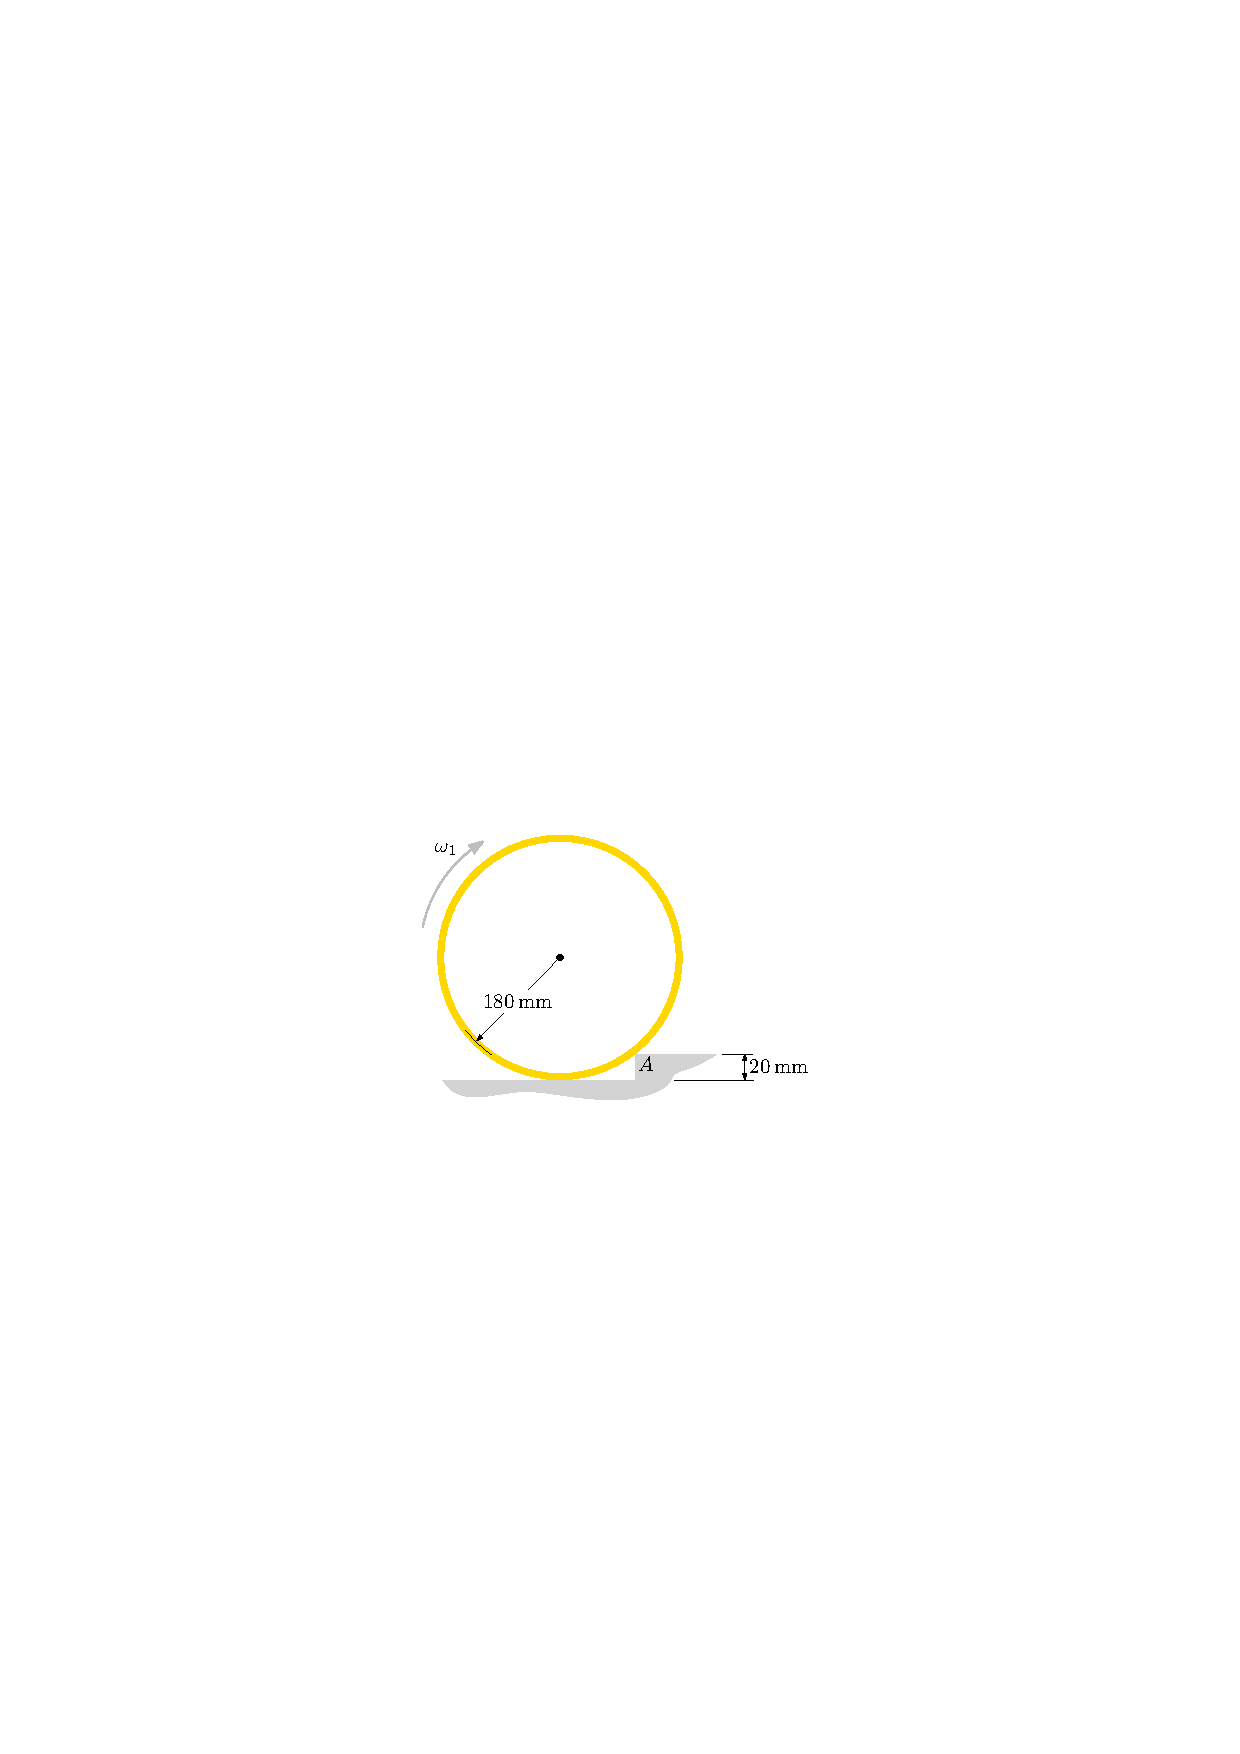
\includegraphics[scale=1.25]{../../images/draw_7_1}
\end{flushright}
